\documentclass[11pt,letterpaper]{article}
\usepackage[T1]{fontenc}
\usepackage[scaled]{helvet}
\renewcommand{\familydefault}{\sfdefault}
\usepackage{amsmath,amssymb}
\usepackage[margin=0.8in,bottom=0.9in]{geometry}
\usepackage[most]{tcolorbox}
\usepackage{tikz}
\usetikzlibrary{calc}
\usepackage{enumitem}
\usepackage{array}
\usepackage{needspace}
\usepackage{fancyhdr}
\usepackage{pifont}

% ---- Palette "F. Bright & Playful" ----
\definecolor{fmtitle}{HTML}{3D2C8D}
\definecolor{fmkey}{HTML}{0096C7}
\definecolor{fmwatch}{HTML}{2BB673}
\definecolor{fmturn}{HTML}{F4A100}
\definecolor{fmmistake}{HTML}{EF476F}
\definecolor{fmnotice}{HTML}{9B5DE5}
\definecolor{fmgray}{HTML}{6B6B6B}

\pagestyle{fancy}
\fancyhf{}
\renewcommand{\headrulewidth}{0pt}
\fancyfoot[C]{\footnotesize\color{fmgray}\textcopyright\ 2026 FangMath. All rights reserved.}
\fancyfoot[R]{\footnotesize\color{fmgray}\thepage}
\setlength{\parindent}{0pt}
\setlength{\parskip}{3pt}

\newcommand{\badge}[1]{\colorbox{fmtitle}{\color{white}\bfseries\small\ #1\ }}
\newcommand{\leveltag}[2]{\colorbox{#1}{\color{white}\bfseries\scriptsize\ #2\ }}
\newcommand{\LE}{\leveltag{fmwatch}{EASY}}
\newcommand{\LM}{\leveltag{fmturn}{MEDIUM}}
\newcommand{\LH}{\leveltag{fmmistake}{HARD}}

\newcommand{\sectionbar}[2]{\needspace{6cm}\par\vspace{4mm}
  \begin{tcolorbox}[enhanced,colback=fmtitle,colframe=fmtitle,arc=2mm,
    left=4mm,top=1.5mm,bottom=1.5mm]
  \color{white}\bfseries\large #1\hfill{\normalsize\mdseries #2}
  \end{tcolorbox}}

\newtcolorbox{keyidea}{enhanced,breakable,colback=white,colframe=fmkey,boxrule=1pt,arc=2mm,
  title={Key Idea},coltitle=fmkey,fonttitle=\bfseries,
  attach boxed title to top left={xshift=4mm,yshift=-2mm},
  boxed title style={colback=white,colframe=fmkey,boxrule=0.9pt}}
\newtcolorbox{watchme}{enhanced,colback=white,colframe=fmwatch,boxrule=1pt,arc=2mm,
  title={Watch Me --- Worked Example},coltitle=fmwatch,fonttitle=\bfseries,
  attach boxed title to top left={xshift=4mm,yshift=-2mm},
  boxed title style={colback=white,colframe=fmwatch,boxrule=0.9pt}}
\newtcolorbox{mistakebox}{enhanced,breakable,colback=white,colframe=fmmistake,boxrule=1pt,arc=2mm,
  title={Common Mistake},coltitle=fmmistake,fonttitle=\bfseries,
  attach boxed title to top left={xshift=4mm,yshift=-2mm},
  boxed title style={colback=white,colframe=fmmistake,boxrule=0.9pt}}
\newtcolorbox{yourturn}{enhanced,breakable,colback=white,colframe=fmturn,boxrule=1pt,arc=2mm,
  title={Your Turn},coltitle=fmturn,fonttitle=\bfseries,
  attach boxed title to top left={xshift=4mm,yshift=-2mm},
  boxed title style={colback=white,colframe=fmturn,boxrule=0.9pt}}
\newtcolorbox{answerbox}[1]{enhanced,breakable,colback=white,colframe=fmwatch,boxrule=1pt,arc=2mm,
  title={#1},coltitle=fmwatch,fonttitle=\bfseries,
  attach boxed title to top left={xshift=4mm,yshift=-2mm},
  boxed title style={colback=white,colframe=fmwatch,boxrule=0.9pt}}

\newcommand{\work}[1]{\par\vspace{#1}}
\setlist[enumerate]{itemsep=2pt,topsep=3pt}

% ---------------- extra boxes ----------------
\newtcolorbox{notebox}{enhanced,breakable,colback=white,colframe=fmnotice,boxrule=1pt,arc=2mm,
  title={Notice},coltitle=fmnotice,fonttitle=\bfseries,
  attach boxed title to top left={xshift=4mm,yshift=-2mm},
  boxed title style={colback=white,colframe=fmnotice,boxrule=0.9pt}}
\newtcolorbox{exbox}{enhanced,colback=white,colframe=fmwatch,boxrule=0.8pt,arc=2mm,
  title={Example},coltitle=fmwatch,fonttitle=\bfseries\small,
  attach boxed title to top left={xshift=4mm,yshift=-2mm},
  boxed title style={colback=white,colframe=fmwatch,boxrule=0.8pt},fontupper=\small}
\newcommand{\topicbar}[1]{\needspace{4.5cm}\par\vspace{5mm}
  \begin{tcolorbox}[enhanced,colback=fmtitle,colframe=fmtitle,arc=2mm,left=4mm,top=1.5mm,bottom=1.5mm]
  \color{white}\bfseries\large #1
  \end{tcolorbox}}
\usepackage{multicol}

% ---------------- practice layout ----------------
\newcommand{\workline}{\par\vspace{7mm}{\color{gray!55}\rule{\linewidth}{0.4pt}}}
\newcommand{\worklines}[1]{\foreach \i in {1,...,#1}{\workline}}
\newcommand{\prob}[3]{\needspace{#3}\par\vspace{3mm}{\color{fmturn}\bfseries #1.}\ #2\par}
\newcommand{\ansline}{\par\vspace{4mm}\hfill\textbf{Answer:}\ \rule{5cm}{0.4pt}\par}
\newcommand{\keyitem}[3]{\needspace{3.2cm}\par\vspace{2mm}
  \begin{tcolorbox}[enhanced,colback=white,colframe=fmwatch!60,boxrule=0.6pt,arc=1.5mm,left=3mm,top=1.5mm,bottom=1.5mm]
  {\color{fmwatch}\bfseries #1.}\quad\small #2\par\vspace{1mm}
  \normalsize\textbf{Answer: #3}
  \end{tcolorbox}}


\usetikzlibrary{arrows.meta}
\providecommand{\iskey}{0}
% fill-in blank: line for students, pink answer in the key
\newcommand{\fb}[2][2.6cm]{\ifnum\iskey=1 \underline{\makebox[#1][c]{\color{fmmistake}\bfseries #2}}\else\underline{\makebox[#1]{}}\fi}
% answer line for practice problems
\newcommand{\pans}[2][3.2cm]{\ifnum\iskey=1 \underline{\makebox[#1][c]{\color{fmmistake}\bfseries #2}}\else\rule{#1}{0.4pt}\fi}
\newcommand{\vid}[1]{{\color{fmgray}\small\textit{\ding{43} Video: #1}}}
\newcommand{\pt}[2]{\fill (#1) circle (2.2pt) node[above=1pt,font=\small]{$#2$};}

\usetikzlibrary{decorations.pathreplacing}
\newcommand{\gridb}[4]{\draw[gray!30,step=1] (#1,#2) grid (#3,#4);\draw[gray!70,-{Stealth}] (#1,0)--(#3+0.4,0);\draw[gray!70,-{Stealth}] (0,#2)--(0,#4+0.4);}
\newcommand{\sdp}[3]{\begin{minipage}[t][2.4cm]{0.48\linewidth}{\color{fmturn}\bfseries #1.}\ #2\par\vfill\hfill \pans[3.6cm]{#3}\end{minipage}}
\newcommand{\sdpw}[3]{\begin{minipage}[t][2.4cm]{0.48\linewidth}{\color{fmturn}\bfseries #1.}\ #2\par\vfill\hfill \pans[5.2cm]{#3}\end{minipage}}
\newcommand{\algp}[3]{\begin{minipage}[t][4.2cm]{0.48\linewidth}{\color{fmturn}\bfseries #1.}\ #2\par\vfill\hfill \pans[4.4cm]{#3}\end{minipage}}
\newcommand{\pair}[2]{\needspace{3.4cm}\noindent #1\hfill #2\par\vspace{2mm}}
\newcommand{\head}[2]{\ifnum\iskey=1 \colorbox{fmwatch}{\color{white}\bfseries\small\ ANSWER KEY\ }\else\badge{#1}\fi\hfill{\small\color{fmgray}Geometry \textperiodcentered\ Lesson #2}\par\vspace{4mm}}
\newcommand{\nameline}{Name: \rule{6cm}{0.4pt}\hspace{1cm}Date: \rule{3.5cm}{0.4pt}\par\vspace{2mm}}
\renewcommand{\vid}[1]{\needspace{4.2cm}{\color{fmgray}\small\textit{\ding{43} Video: #1}}}
\begin{document}
\head{WATCH \& FILL IN}{1.6}
{\color{fmtitle}\LARGE\bfseries Constructions --- Notes\ifnum\iskey=1 \ --- Answer Key\fi}\par\vspace{1mm}
{\color{fmgray}Watch the video and fill in each blank. Pause when you see ``Your turn.''}\par\vspace{3mm}
\nameline

\vid{The two tools}
\begin{keyidea}\textbf{Compass:} draws \fb[2.8cm]{circles and arcs}, and copies a \fb[1.6cm]{length}.\par\vspace{1mm}
\textbf{Straightedge:} draws straight lines --- \fb[2.6cm]{no measuring}!\par\vspace{2mm}
Four basics: copy a segment, copy an angle, bisect a \fb[1.8cm]{segment}, bisect an \fb[1.6cm]{angle}.\end{keyidea}

\vid{Bisect a segment (find its midpoint)}
\begin{keyidea}\begin{minipage}[c]{0.38\linewidth}\centering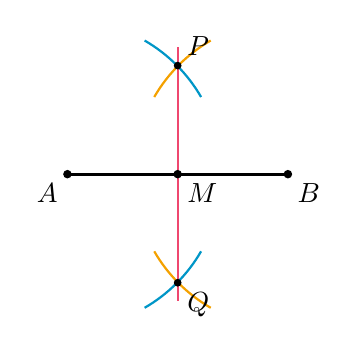
\begin{tikzpicture}[scale=0.7]
\draw[very thick] (0,0)--(4,0);\fill (0,0) circle(2.2pt) node[below left]{$A$} (4,0) circle(2.2pt) node[below right]{$B$};
\draw[fmkey,thick] (0,0) ++(30:2.8) arc (30:60:2.8);\draw[fmkey,thick] (0,0) ++(-30:2.8) arc (-30:-60:2.8);
\draw[fmturn,thick] (4,0) ++(150:2.8) arc (150:120:2.8);\draw[fmturn,thick] (4,0) ++(-150:2.8) arc (-150:-120:2.8);
\draw[fmmistake,thick] (2,2.3)--(2,-2.3);\fill (2,1.97) circle(2pt) node[above right]{$P$} (2,-1.97) circle(2pt) node[below right]{$Q$} (2,0) circle(2.2pt) node[below right]{$M$};\end{tikzpicture}\end{minipage}\hfill
\begin{minipage}[c]{0.58\linewidth}\textbf{1.} From $A$: open the compass \fb[2.6cm]{more than half} of $AB$. Draw arcs above and below.\par\vspace{1mm}
\textbf{2.} From $B$: use the \fb[1.4cm]{same} width. Arcs above and below.\par\vspace{1mm}
\textbf{3.} The arcs cross at \fb[0.8cm]{$P$} and \fb[0.8cm]{$Q$}.\par\vspace{1mm}
\textbf{4.} Line $PQ$ is the \fb[4cm]{perpendicular bisector}. It meets $\overline{AB}$ at the \fb[1.8cm]{midpoint} $M$.\end{minipage}\end{keyidea}

\vid{Watch out}
\begin{mistakebox}Keep the compass width the \fb[1.4cm]{same} for both arcs, and open it to \fb[2.6cm]{more than half} of $AB$ --- otherwise the arcs won't \fb[1.4cm]{cross}.\end{mistakebox}

\vid{Bisect an angle}
\begin{keyidea}\begin{minipage}[c]{0.38\linewidth}\centering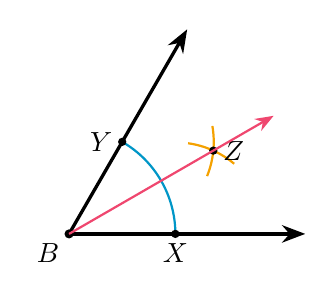
\begin{tikzpicture}[scale=0.75]
\draw[very thick,-{Stealth}] (0,0)--(4,0);\draw[very thick,-{Stealth}] (0,0)--(60:4);\fill (0,0) circle(2.2pt) node[below left]{$B$};
\draw[fmkey,thick] (1.8,0) arc (0:60:1.8);\fill (1.8,0) circle(2pt) node[below]{$X$} (60:1.8) circle(2pt) node[left]{$Y$};
\draw[fmturn,thick] (1.8,0) ++(50:1.55) arc (50:82:1.55);\draw[fmturn,thick] (60:1.8) ++(-22:1.55) arc (-22:10:1.55);
\fill (30:2.821) circle(2pt) node[right]{$Z$};\draw[fmmistake,thick,-{Stealth}] (0,0)--(30:4);\end{tikzpicture}\end{minipage}\hfill
\begin{minipage}[c]{0.58\linewidth}\textbf{1.} An arc from the vertex $B$ crosses both sides at \fb[0.8cm]{$X$} and \fb[0.8cm]{$Y$}.\par\vspace{1mm}
\textbf{2.} Same width from $X$ and from $Y$: the arcs meet at \fb[0.8cm]{$Z$}.\par\vspace{1mm}
\textbf{3.} Ray $BZ$ \fb[1.6cm]{bisects} the angle: two \fb[1.4cm]{equal} halves.\end{minipage}\end{keyidea}

\vid{Copy a segment}
\begin{keyidea}Set the compass to \fb[1.2cm]{$AB$}. Put the point on $C$ and draw an arc across the ray. Where it crosses is $D$.\par\vspace{1mm}
Now $CD$ \fb[1cm]{$=$} $AB$ --- copied without \fb[2cm]{measuring}.\end{keyidea}

\vid{Your turn}
\begin{yourturn}You want to bisect a segment that is $8$ cm long. Which compass width works: $3$ cm or $5$ cm?\par\vspace{2mm}
Answer: \fb[1.4cm]{$5$ cm}, because it must be more than half of $8$ cm, which is \fb[1.4cm]{$4$ cm}.\par\vspace{1mm}
With $3$ cm the arcs from $A$ and $B$ never \fb[1.4cm]{meet}.\end{yourturn}
\end{document}
